\chapter{Prezentacja warstwy użytkowej projektu}
\label{cha:warstwa_uzytkowa}

\section{Opis szaty graficznej}

Interfejs graficzny aplikacji został zaprojektowany z myślą o przejrzystości i intuicyjnej obsłudze. Zastosowano nowoczesną, minimalistyczną stylistykę z przewagą odcieni szarości, bieli i fioletu. Wszystkie ikony użyte w aplikacji pochodzą z serwisu \textbf{Icons8}, natomiast tło oraz logo zostały przygotowane na zamówienie, specjalnie na potrzeby projektu.

\section{Prezentacja głównych widoków interfejsu użytkownika}

\subsection{Okno logowania}

Ekran logowania jest pierwszym widokiem wyświetlanym użytkownikowi po uruchomieniu aplikacji. Składa się z formularza zawierającego pola do wpisania nazwy użytkownika i hasła, przycisku logowania oraz opcjonalnego komunikatu błędu w przypadku nieprawidłowych danych. Widok jest klarowny, aby nie rozpraszać użytkownika i umożliwić szybkie przejście do dalszej pracy.
\begin{figure}[H]
    \centering
    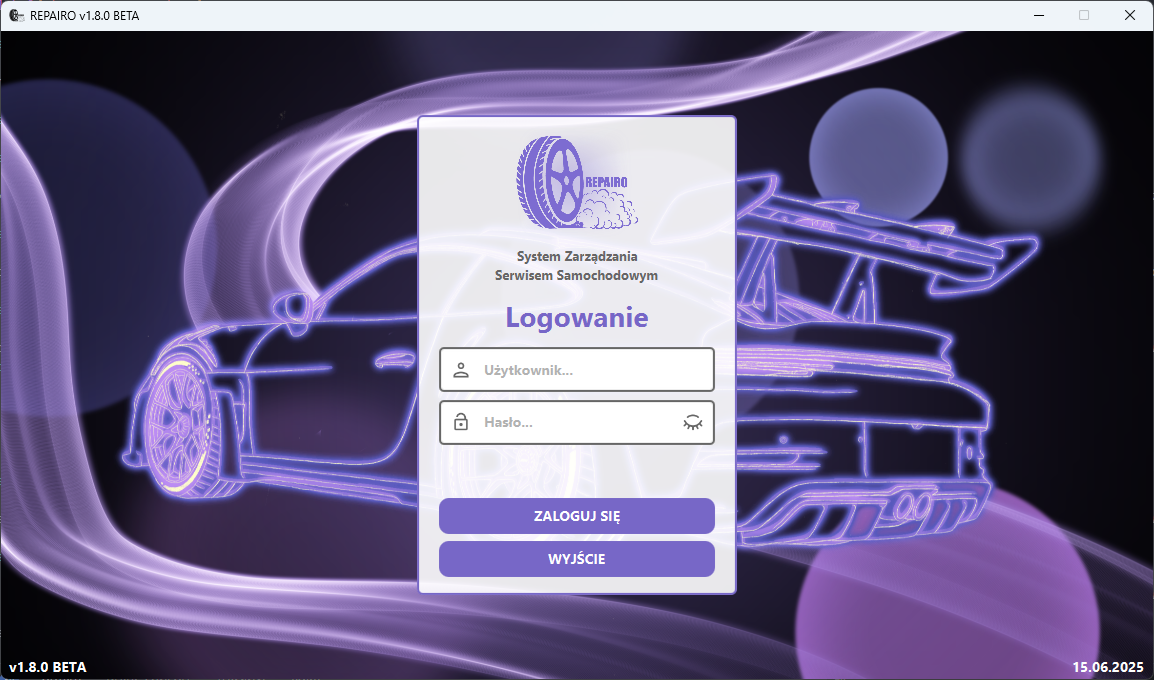
\includegraphics[width=\textwidth,height=0.6\textheight,keepaspectratio]{figures/oknoLogowania.png}
    \caption{Okno logowania}
    \label{fig:oknoLogowania}
\end{figure}

\newpage
\subsection{Główne okno interfejsu}

Po zalogowaniu użytkownik zostaje przeniesiony do głównego panelu aplikacji. Widok ten składa się z górnego paska menu, menu bocznego z listą zakładek oraz dynamicznej przestrzeni roboczej (tzw. \textit{main pane}), w której wyświetlane są odpowiednie komponenty w zależności od wybranej zakładki.
\begin{figure}[H]
    \centering
    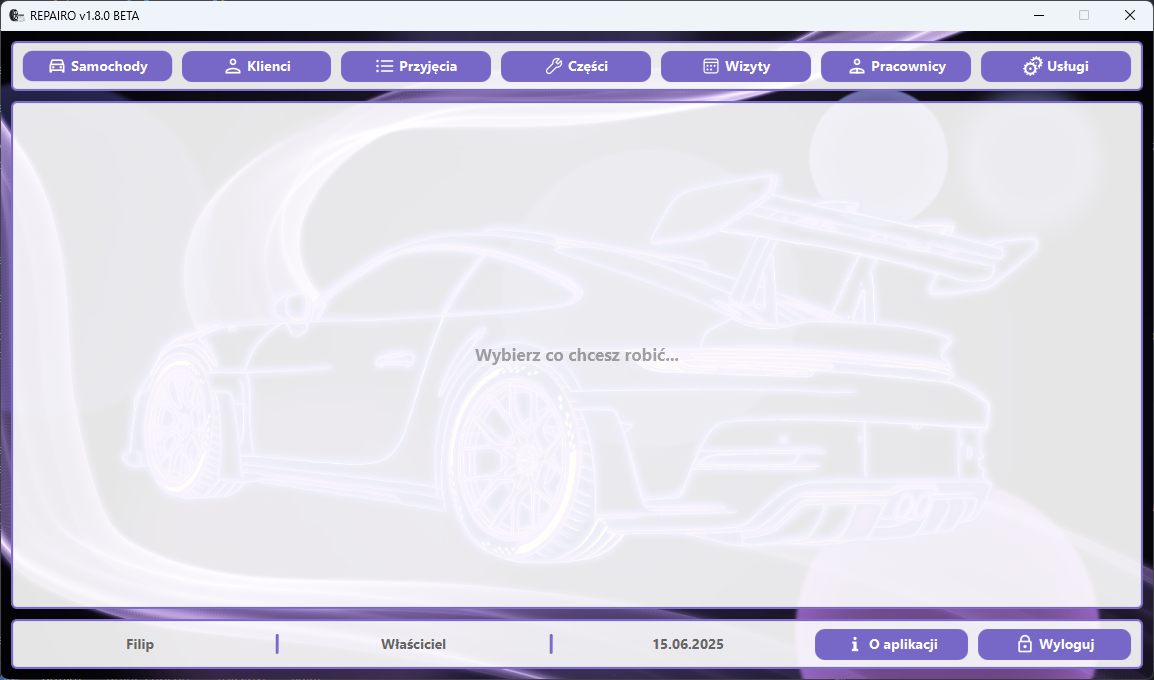
\includegraphics[width=0.8\textwidth,height=0.8\textheight,keepaspectratio]{figures/glowneokno.png}
    \caption{Główne okno interfejsu}
    \label{fig:glownyPanel}
\end{figure}


\subsection{Okno zarządzania samochodami}
Widok umożliwia przeglądanie, dodawanie informacji o pojazdach znajdujących się w bazie danych na podstawie wybranych danych z list rozwijanych.
\begin{figure}[H]
    \centering
    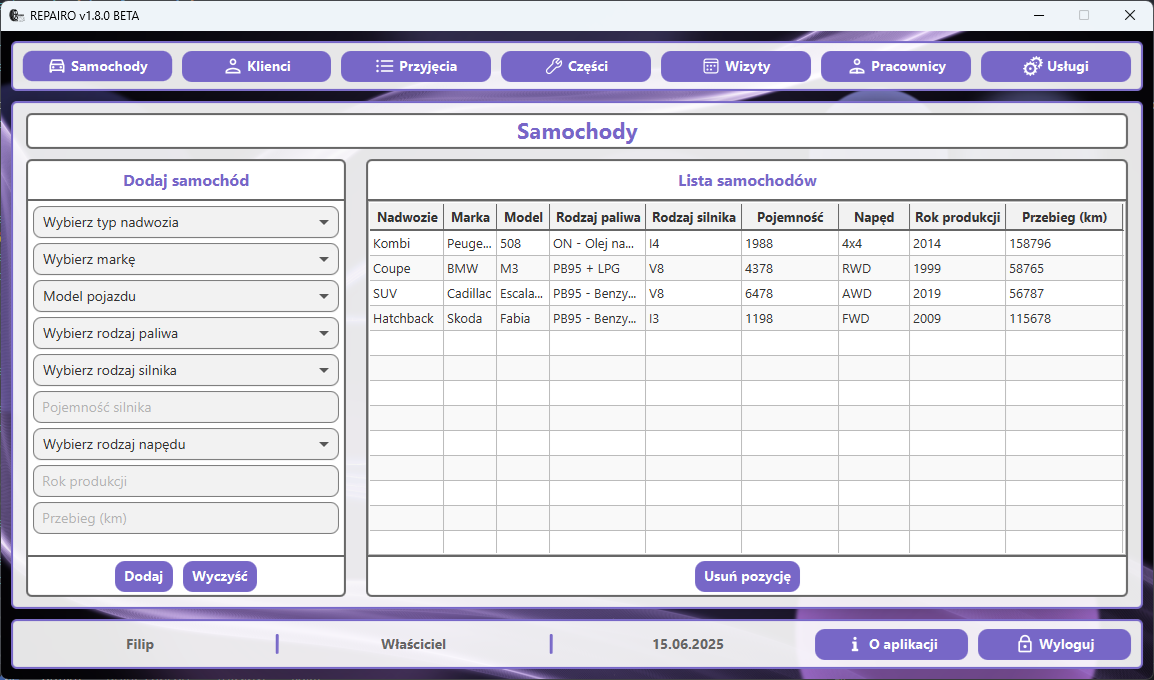
\includegraphics[width=0.8\textwidth,height=0.8\textheight,keepaspectratio]{figures/samochody.png}
    \caption{Okno zarządzania samochodami}
    \label{fig:oknoSamochody}
\end{figure}

\newpage
\subsection{Okno zarządzania klientami}
Panel pozwala na zarządzanie danymi kontaktowymi klientów oraz ich typami (np. osoba prywatna lub firma). Można tu również dodać informację takie jak numer telefonu czy adres e-mail, co ułatwia kontakt z klientami w przyszłości.

\begin{figure}[H]
    \centering
    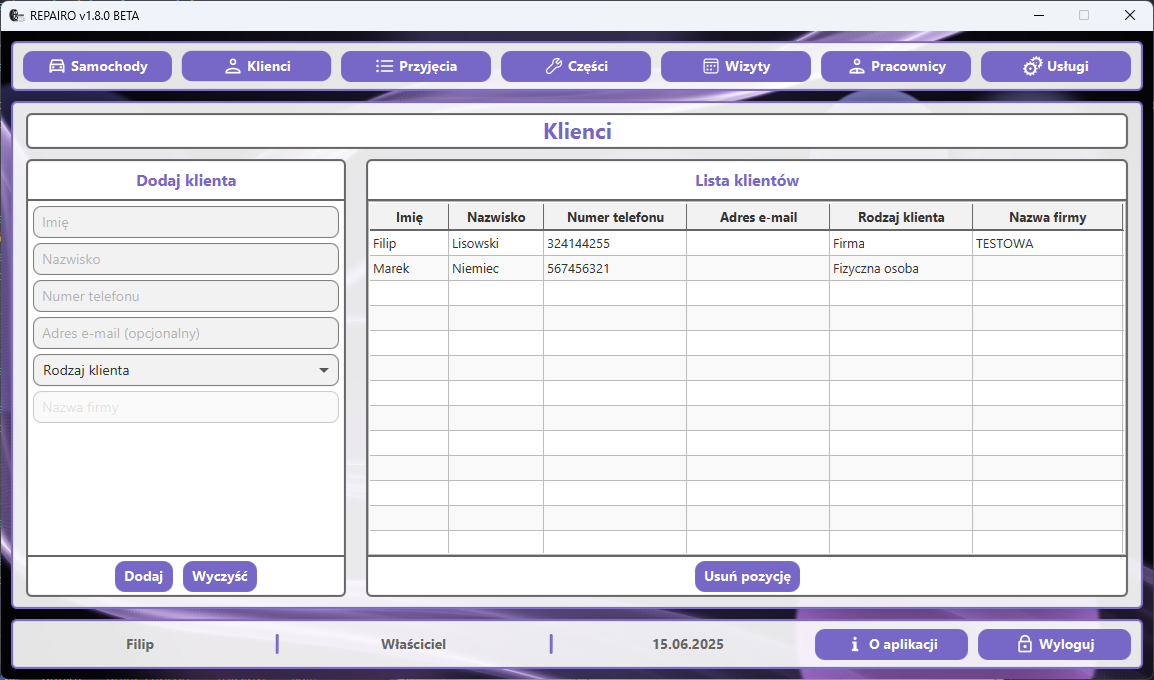
\includegraphics[width=0.8\textwidth,height=0.8\textheight,keepaspectratio]{figures/klienci.png}
    \caption{Okno zarządzania klientami}
    \label{fig:oknoKlienci}
\end{figure}


\subsection{Okno zarządzania przyjęciami}
W tym widoku możliwe jest tworzenie nowych zleceń serwisowych oraz przypisywanie ich do klientów, pojazdów oraz pracowników. Dodatkowo, użytkownik może dopisać rodzaj oraz ilość użytych części.

\begin{figure}[H]
    \centering
    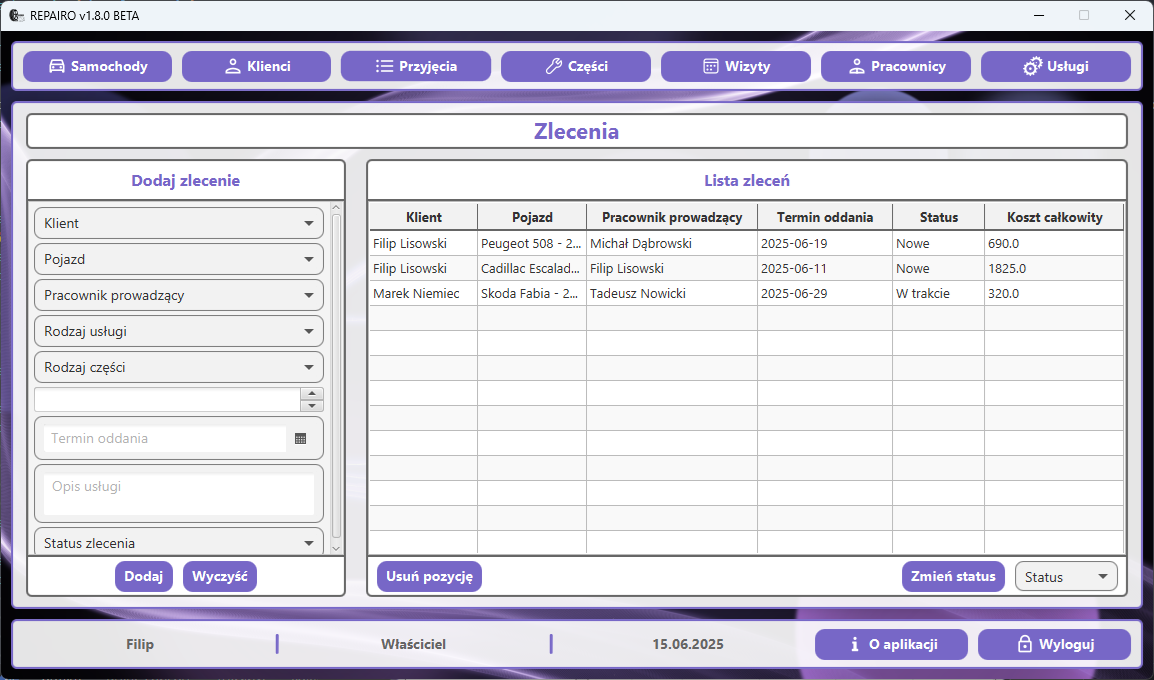
\includegraphics[width=0.8\textwidth,height=0.8\textheight,keepaspectratio]{figures/przyjecia.png}
    \caption{Okno zarządzania przyjęciami}
    \label{fig:oknoPrzyjecia}
\end{figure}

\newpage
\subsection{Okno zarządzania częściami}
Użytkownik ma możliwość dodawania i usuwania części zamiennych dostępnych w warsztacie. Pondadto można przeglądać ich stany magazynowe oraz przypisane do nich ceny.

\begin{figure}[H]
    \centering
    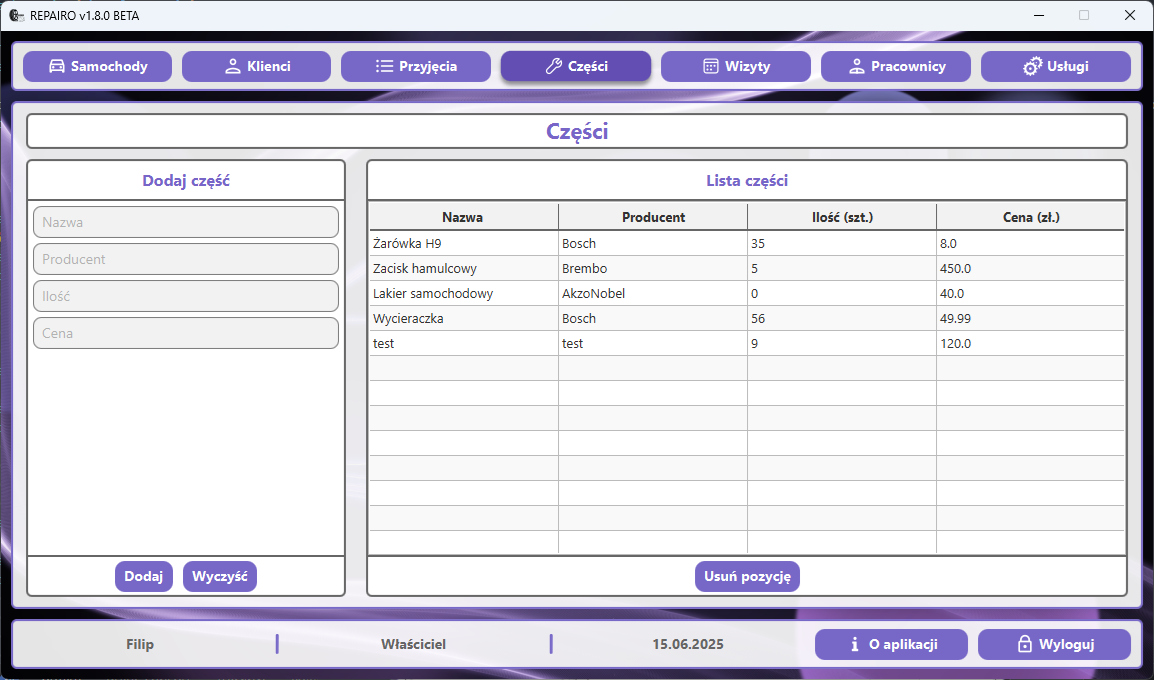
\includegraphics[width=0.8\textwidth,height=0.8\textheight,keepaspectratio]{figures/czesci.png}
    \caption{Okno zarządzania częściami}
    \label{fig:oknoCzesci}
\end{figure}

\subsection{Okno zarządzania wizytami}
Panel prezentuje wizyty, daty zakończenia oraz aktualne statusy realizacji zleceń. Dodatkowo, można przemieszczać się pomiędzy miesiącami, aby przeglądać wizyty z różnych okresów. Widok ten jest kluczowy dla monitorowania bieżących i przyszłych zleceń w warsztacie.
Na kolor czerwony zaznaczono termin oddania pojazdu. Na kolor niebieski zaznaczono aktualny dzień tygodnia.
\begin{figure}[H]
    \centering
    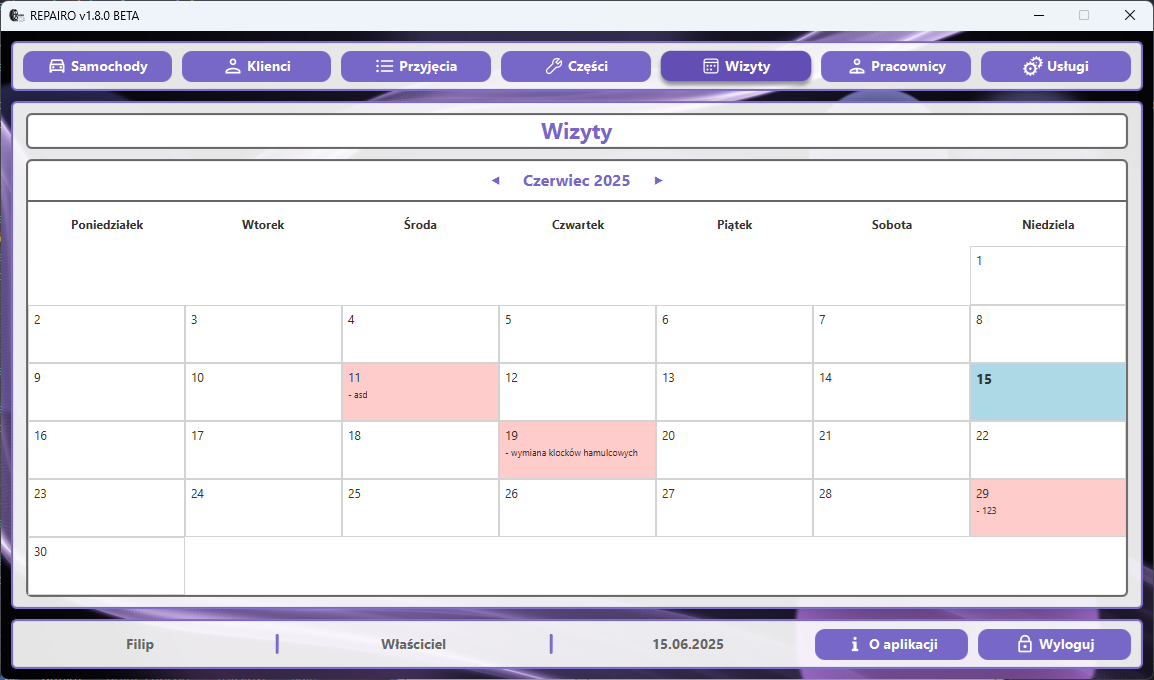
\includegraphics[width=0.8\textwidth,height=0.8\textheight,keepaspectratio]{figures/wizyty.png}
    \caption{Okno zarządzania wizytami}
    \label{fig:oknoWizyty}
\end{figure}


\newpage
\subsection{Okno zarządzania pracownikami}
Umożliwia jedynie wyświetlanie listy pracowników (na potrzeby projektu założono, że zarządzanie pracownikami odbywa się poprzez system bazodanowy). 

\begin{figure}[H]
    \centering
    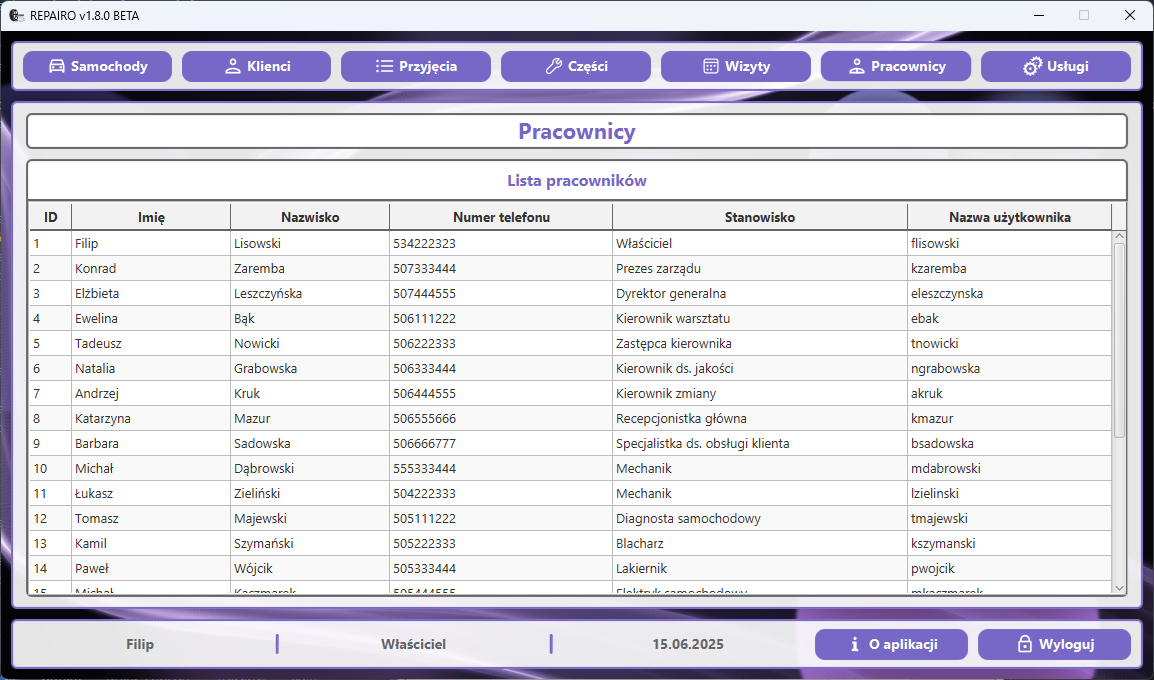
\includegraphics[width=0.8\textwidth,height=0.8\textheight,keepaspectratio]{figures/pracownicy.png}
    \caption{Okno zarządzania pracownikami}
    \label{fig:oknoPracownicy}
\end{figure}


\subsection{Okno zarządzania usługami}
Widok służy do dodawania i modyfikowania usług oferowanych przez warsztat, wraz z przypisanym kosztem.

\begin{figure}[H]
    \centering
    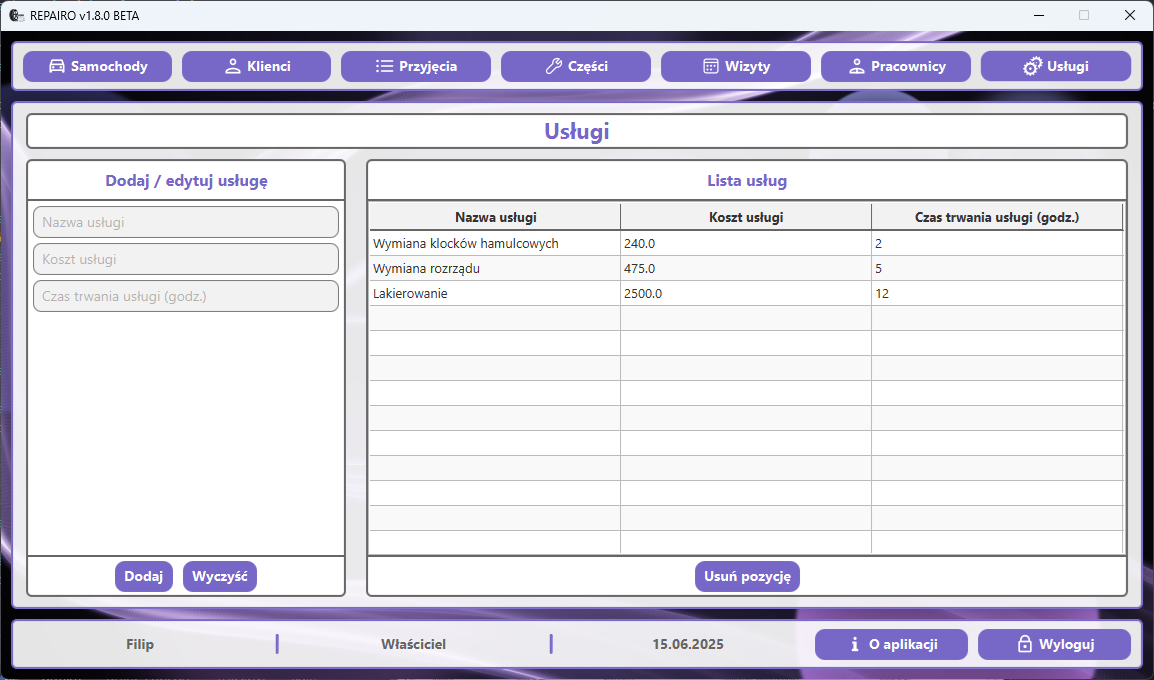
\includegraphics[width=0.8\textwidth,height=0.8\textheight,keepaspectratio]{figures/uslugi.png}
    \caption{Okno zarządzania usługami}
    \label{fig:oknoUslugi}
\end{figure}


\newpage
\subsection{Okno wyświetlania informacji o aplikacji}
W tym miejscu użytkownik znajdzie informacje o wersji systemu, autorze projektu oraz danych kontaktowych.

\begin{figure}[H]
    \centering
    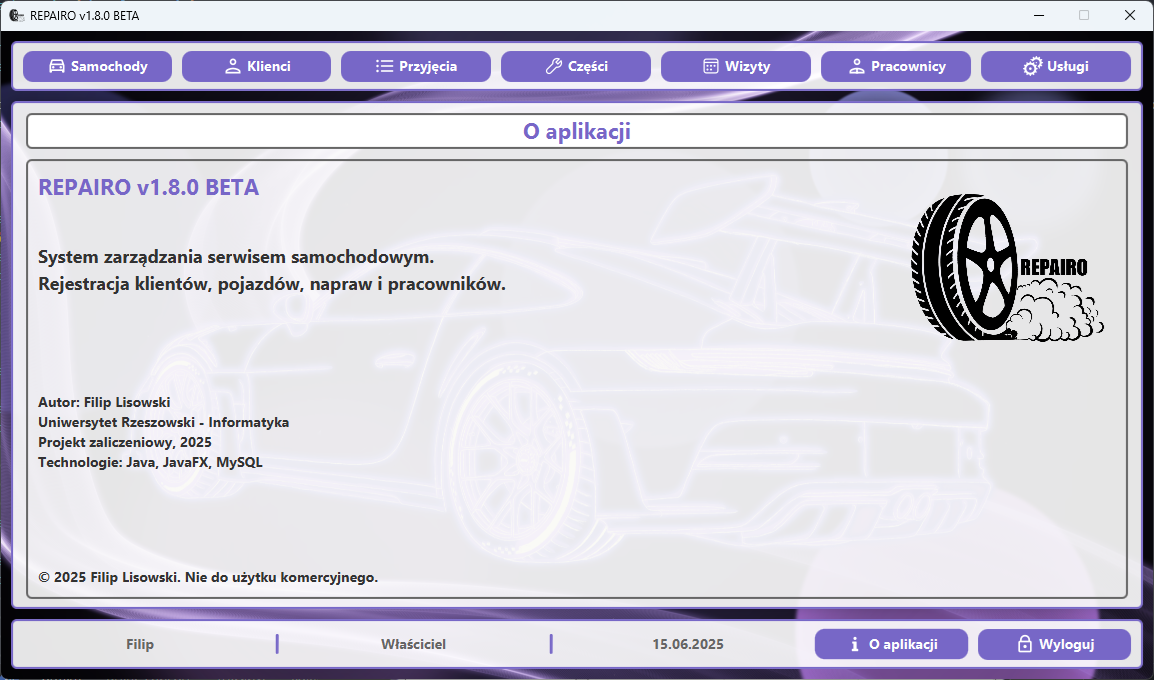
\includegraphics[width=0.8\textwidth,height=0.8\textheight,keepaspectratio]{figures/info.png}
    \caption{Okno informacji o aplikacji}
    \label{fig:oknoInfo}
\end{figure}



\newpage
\section{Mechanizm alertów systemowych}

W aplikacji zastosowano dedykowany mechanizm powiadomień systemowych, który informuje użytkownika o sukcesie lub błędzie operacji. Powiadomienia te wyświetlane są w formie wyskakujących okien typu \textit{popup}, zawierających ikonę, krótki komunikat.
Poniżej przedstawiono przykładowe komunikaty wyświetlane użytkownikowi. Informują one o konieczności potwierdzenia wylogowania lub zamknięcia aplikacji, a także ostrzegają o błędnym wprowadzeniu danych.
\begin{figure}[H]
    \centering
    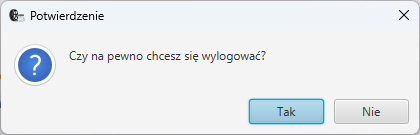
\includegraphics[width=0.8\textwidth,height=0.8\textheight,keepaspectratio]{figures/wylogowanie.png}
    \caption{Alert potwierdzenia wylogowania}
    \label{fig:oknoWylogowanie}
\end{figure}

\begin{figure}[H]
    \centering
    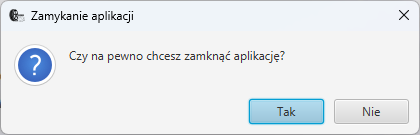
\includegraphics[width=0.8\textwidth,height=0.8\textheight,keepaspectratio]{figures/zamknij.png}
    \caption{Alert potwierdzenia wyjścia z aplikacji}
    \label{fig:oknoZamknij}
\end{figure}

\begin{figure}[H]
    \centering
    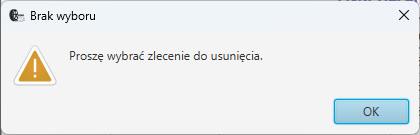
\includegraphics[width=0.8\textwidth,height=0.8\textheight,keepaspectratio]{figures/zlywybor.png}
    \caption{Alert o błędnym wprowadzeniu danych}
    \label{fig:oknoZlyWybor}
\end{figure}
Mechanizm ten został zaimplementowany w sposób uniwersalny, dzięki czemu może być łatwo wykorzystywany w dowolnym komponencie aplikacji.
